\ifxHPTDC{
	\newcommand{\device}{\cronvar{\prefix manager}{*xhptdc8\tu mgr}}
	\newcommand{\deviceindex}{\device, \cronvar{int}{index}}
	\newcommand{\deviceconfig}{\device}
	\newcommand{\initparameters}{xhptdc8\tu manager\tu init\tu parameters}
}{
	\newcommand{\device}{\cronvar{\prefix device}{*device}}
	\newcommand{\deviceindex}{\device}
	\newcommand{\deviceconfig}{\deviceindex}
	\newcommand{\initparameters}{\prefix init\tu parameters}
}

The API is a DLL with C linkage.\par

The functions provided by the driver are declared in \textsf{\txh{TimeTagger4}{xTDC4}{xHPTDC8}\tu interface.h} 
which must be included by your source code.
You must tell your compiler to link with the file \textsf{xhptdc8\tu driver.lib} 
or the corresponding 64 bit version \textsf{xhptdc8\tu driver\tu 64.lib}.
When running your program the dynamic link library containing the actual driver code must reside in the same directory as your executable. 
The file for the DLL is called \textsf{\prefix driver.dll} for x86 and \textsf{\prefix driver\tu 64.dll} for x64.

All these files are provided with the driver installer that can be downloaded from the product website \url{https://www.cronologic.de}. 
By default the installer will place the files into the directory 
\textsf{C:\filesep program files\filesep cronologic\filesep \deviceName\filesep driver}.

\ifxHPTDC{
	There exist an open source community project that intends to provide some convenient extensions to the driver, code examples 
	and wrappers to make the driver usable with various programming languages like Python and LabView. 
	The project is hosted at \url{https://github.com/cronologic-de/xhptdc8_babel}.
}{}

 
\section{Constants}
\ifxHPTDC{
	\crondef{XHPTDC8\tu MANAGER\tu DEVICES\tu MAX 8}\\
	The maximum number of boards supported by the device manager.

	\ttdef{TDC\tu CHANNEL\tu COUNT 8}\\
	The number of TDC input channels.\par

	\ttdef{GATE\tu COUNT 8}\\
	The number of gating blocks. One for each TDC input.\par

	 \ttdef{TIGER\tu COUNT 9}\\
	The number of timing generators. One for each TDC input and one for the adc trigger.\par

	 \ttdef{TRIGGER\tu COUNT 16}\\
	The number of potential trigger sources for the timing generators. One for each TDC input 
	\ifxHPTDC{}{, one for the Start input} plus some specials. 
	 See Section~\ref{structtrigger} for details.\par

}{ 
	\ttdef{CHANNEL\tu COUNT 4}\\
	The number of TDC input channels.\par

	 \ttdef{TIGER\tu COUNT 5}\\
	The number of timing generators. One for each TDC input and one for the start input.\par

	 \ttdef{TRIGGER\tu COUNT 16}\\
	The number of potential trigger sources for the timing generators. One for each TDC input, one for the Start input plus some specials. 
	 See Section~\ref{cp:tigerblock} for details.\par
}

\ttdef{OK 0}\\
Error codes are set by the API functions to this value if there has been no error. Other error codes can be found in \textsf{xHPTDC8\tu interface.h}\par

\section{Driver Information}

	Even if there is no board present the driver revision can be queried using these functions.

	\ttvar{int}{get\tu driver\tu revision()}\\
	Returns the driver version, same format as \textsf{\prefix static\tu info.driver\tu revision}. 
	This function does not require a \deviceName\ board to be present.

	\ttvar{const char*}{get\tu driver\tu revision\tu str()}\\
	Returns the driver version including SVN build revision as a string. 

	\ttvar{int}{count\tu devices(}\cronvar{int}{*error\tu code}, \cronvar{char}{**error\tu message)}\\
	\label{countdevices}
	Returns the number of boards present in the system that are supported by this driver.\par


\section {Initialization}

		\ttvar{int}{close(}\device )\\
		Finalizes the driver for this device.

		\ttvar{int}{get\tu default\tu init\tu parameters(}\cronvar{\initparameters}{ *init)}\\
		Sets up the standard parameters. Gets a set of default parameters for \textsf{\prefix init()}. 
		This must always be used to initialize the \textsf{\initparameters} structure before modifying it 
		and passing it to \textsf{\prefix init}.\par

		\cronvar{\prefix \ifxHPTDC{manager}{device} *}{\prefix init(}\cronvar{\initparameters}{*params}, \\ 
		\cronvar{int}{*error\tu code}, \cronvar{char}{**error\tu message)}\\
		Opens and initializes the \deviceName. 
		\ifxHPTDC{boardss}{board with the given index}. \\
		\textsf{error\tu code} shall point to an integer where the driver can write the the error code. \\
		\textsf{error\tu message} must point to a pointer to char. 
		The driver will allocate a buffer for zero terminated error message and store the address of the buffer in the location provided by the user.\par

		The paramter \textsf{params} is a structure of type \textsf{\initparameters} that must be completely initialized.\par

%%%%%%%%%%%%%%%%% struct init_parameters

		\subsection{Structure \initparameters}
			\cronvar{int}{version}\\
			The version number. Must be set to \textsf{\PREFIX API\tu VERSION}.\par

			\ifxHPTDC{}{
				\cronvar{int}{card\tu index}\\
				The index in the list of \deviceName\ boards that should be initialized.\\
				There might be multiple boards in the system that are handled by this driver as reported by \textsf{\prefix count\tu devices}. This index selects one of them. Boards are enumerated depending on the PCIe slot. 
				The lower the bus number and the lower the slot number the lower the card index.\par

				\cronvar{int}{board\tu id}\\
				the global index in all cronologic devices.\\
				This 8 bit number is filled into each packet created by the board and is useful if data streams of multiple boards will be merged. If only \deviceName\ cards are used this number can be set to the \textsf{card\tu index}. 
				If boards of different types that use a compatible data format are used in a system each board should get a unique id.
				Can be changed with \textsf{int \prefix set\tu board\tu id\allowbreak(\prefix device *device, int board\tu id)}.\par
			}

			\cronvar{\longlong}{buffer\tu size\ifxHPTDC{}{[8]}}\\
			The minimum size of the DMA buffer.\\
			If set to 0 the default size of 16~MByte is used. 
			\ifxHPTDC{}{For the \deviceName\ only the first entry is used.}\par

			\ifxHPTDC{}{
				\cronvar{int}{buffer\tu type}\\
				The type of buffer. Must be set to 0.
				\begin{description}
					\item[]  \ttdef{BUFFER\tu ALLOCATE   0}
					\item[]  \ttdef{BUFFER\tu USE\tu PHYSICAL   1}  // unsupported
				\end{description}
			

				\cronvar{\longlong}{buffer\tu address}\\
				This is set by \prefix init() to the start address of the reserved memory.\\ 
				The buffers will be allocated with the sizes given above. Make sure that the memory is large enough.\par
			}

			\cronvar{int}{variant}\\
			Set to 0. Can be used to activate future device variants such as different base frequencies.\par

			\cronvar{int}{device\tu type}\\
			A constant for the different devices of cronologic \textsf{CRONO\tu DEVICE\tu *}.\\
			Initialized by \textsf{\prefix get\tu default\tu init\tu parameters()}. This value is identical to the PCI Device ID. Must be left unchanged.

			\begin{tabular}{ll}
				\crondef{CRONO\tu DEVICE\tu HPTDC}       & 0x1 \\
				\crondef{CRONO\tu DEVICE\tu NDIGO5G}     & 0x2 \\
				\crondef{CRONO\tu DEVICE\tu NDIGO250M}   & 0x4 \\
				\crondef{CRONO\tu DEVICE\tu xTDC4}       & 0x6 \\
				\crondef{CRONO\tu DEVICE\tu TIMETAGGER4} & 0x8 \\
				\crondef{CRONO\tu DEVICE\tu XHPTDC8}     & 0xC \\
				\crondef{CRONO\tu DEVICE\tu NDIGO6}      & 0xD \\
			\end{tabular}

			\cronvar{int}{dma\tu read\tu delay}\\
			The update delay of the write pointer after a packet has been sent over PCIe. Specified in multiples of 16~ns.
			Should not be changed by the user.\par

			\ifxHPTDC{
				\cronvar{crono\tu bool\tu t}{multiboard}\\
				Set if multiple devices shall be synchronized. Also sets the clock source to external.\par
	
				\cronvar{crono\tu bool\tu t}{use\tu ext\tu clock}\\
				If set use the external 10 MHz reference on J2, otherwise the internal clock source is used. 
				When \textsf{multiboard} is set this parameter is ignored and the external clock is used. \par

				\cronvar{crono\tu bool\tu t}{ignore\tu calibration}\\
				Leave at false to use device calibration data.\par
		
			}{
				\cronvar{int}{use\tu ext\tu clock}\\
				If set to 1 use external 10 MHz reference. If set to 0 use internal reference.\par	
			}
	

	
	% info structures
	\section{Status Information}
	

\subsection{Functions for Information Retrieval}
    The driver provides functions to retrieve detailed information on the board type, its configuration, settings and state. 
    The information is split according to its scope and the computational requirements to query the information from the board.
    
    \ifxHPTDC{
        The information is provided on a per board basis. The parameter \textsf{index} selects which board is queried.
    }{}

    \ttvar{int}{get\tu device\tu type}(\device)\\
    Returns the type of the device as \textsf{CRONO\tu DEVICE\tu \txh{TIMETAGGER4}{XTDC4}{XHPTDC8}}.\par

    \ttvar{const char*}{get\tu last\tu error\tu message(\device)}\\
    Returns most recent error message.\par

    \ttvar{int}{get\tu fast\tu info(}\deviceindex, \lb\cronvar{\prefix fast\tu info}{*info)}\\
    Returns fast dynamic information.\\
    This call gets a structure that contains dynamic information that can be obtained within a few microseconds.\par

    \ttvar{int}{get\tu param\tu info(}\deviceindex, \lb\cronvar{\prefix param\tu info}{*info)}\\
    Returns configuration changes.\\
    Gets a structure that contains information that changes indirectly due to configuration changes.\par


    \ttvar{int}{get\tu static\tu info(}\deviceindex, \lb\cronvar{\prefix static\tu info}{*info)}\\
    Contains static information.\\
    Gets a structure that contains information about the board that does not change during run time.\par 

   \ifxHPTDC{
        \ttvar{int}{get\tu temperature\tu info(}\deviceindex, \lb\cronvar{\prefix temperature\tu info}{*info)}\\
        Get temperature measurements from multiple sources on the board.

        \ttvar{int}{get\tu clock\tu info(}\deviceindex, \lb\cronvar{\prefix clock\tu info}{*info)}\\
        Get information on clocking configuration an status.

        \ttvar{const char *}{device\tu state\tu to \tu str(}\cronvar{int state)}\\
        Convert the state value from \textsf{\prefix fast\tu info.state} into a human readable string. 
   }{   
        \ttvar{int}{get\tu slow\tu info(}\deviceindex, \lb\cronvar{\prefix slow\tu info}{*info)}\\
        Returns slow dynamic information.\\
        The data reported in this structure requires milliseconds to be obtained. 
        The application should only call it in situations where the program flow can be blocked as long.\par
   } 

%%%%%%%%%%%%%%%%% static info

\subsection{Structure \prefix static\tu info}

This structure contains information about the board that does not change during run time. It is provided by the function \textsf{\prefix get\tu static\tu info}.\par

\cronvar{int}{size}\\
The number of bytes occupied by the structure.

\cronvar{int}{version}\\
A version number that is increased when the definition of the structure is changed. The increment can be larger than one to match driver version numbers or similar. Currently only version 0 is defined.\par

\cronvar{int}{board\tu id}\\
ID of the board.\\
\ifxHPTDC{
    All \deviceName\ boards in the system are numbered according in order of their serial numbers starting at zero.
    The channel A of a board has channel number $board\_id \cdot 10$. \par
}{}

\cronvar{int}{driver\tu revision}\\
Encoded version number for the driver.\\
The lower three bytes contain a triple level hierarchy of version numbers, e.g. 0x010103 encodes version 1.1.3.\\
The versionen adheres to the Semantic Versioning scheme as defined at \href{https://semver.org}{https://semver.org}. A change in the first digit generally requires a recompilation of user applications. 
Changes in the second digit denote significant improvements or changes that don't break compatibility 
and the third digit increments with minor bug fixes and similar updates that do not affect the API.\par

\cronvar{int}{driver\tu build\tu revision}\\
The build number of the driver according to cronologic's internal versioning system.

\cronvar{int}{firmware\tu revision}\\
Revision number of the FPGA configuration.

\cronvar{int}{board\tu revision}\\
Board revision number.\\
The board revision number can be read from a register. It is a four-bit number that changes when the schematic of the board is changed. This should match the revision number printed on the board.

\cronvar{int}{board\tu configuration}\\
Describes the schematic configuration of the board.\\
The same board schematic can be populated in multiple variants. This is a four bit-code that can be read from a register.

\cronvar{int}{subversion\tu revision}\\
Subversion revision id of the FPGA configuration source code.

\txh{
    \cronvar{int}{chip\tu id}\\
    Reserved.
}{
    \cronvar{int}{chip\tu id}\\
    16 bit factory ID of the TDC chip.
}{
    \cronvar{int}{chip\tu id[2]}\\
    16 bit factory ID for each of the TDC chips.
}\par

\cronvar{int}{board\tu serial}\\
Serial number.\\
With year and running number in 8.24 format. The number is identical to the one printed on the silvery sticker on the board.\par

\cronvar{unsigned int}{flash\tu serial\tu high}\\
\cronvar{unsigned int}{flash\tu serial\tu low}\\
64-bit manufacturer serial number of the flash chip

\cronvar{crono\tu bool\tu t}{flash\tu valid}\\
If not 0 the driver found valid calibration data in the flash on the board and is using it.\par

\cronvar{int}{calibration\tu date}\\
DIN EN ISO 8601 string YYYY-MM-DD HH:DD describing the time when the card was calibrated.

%%%%%%%%%%%%%%%%%%%%%%%% param info

\subsection{Structure \prefix param\tu info}
This struct contains configuration changes provided by \textsf{\prefix get\tu param\tu info()}.

\cronvar{int}{size}\\
The number of bytes occupied by the structure. \par

\cronvar{int}{version}\\
A version number that is increased when the definition of the structure is changed. The increment can be larger than one to match driver version numbers or similar. Currently only version 0 is defined.\par


\cronvar{double}{binsize}\\
Bin size (in ps) of the measured TDC data.

\ifxHPTDC{}{ %board ID is found in the static_info structure.
    \cronvar{int}{board\tu id}\\
    Board ID.\\
    The board uses this ID to identify itself in the output data stream. The ID takes values between 0 and 255.\par
}

\cronvar{int}{channels}\\
Number of TDC channels of the board.\\
Returns \ifxHPTDC{8}{4}.\par

\cronvar{int}{channel\tu mask}\\
Bit assignment of each enabled input channel.\\
Bit $0 \leq n < \ifxHPTDC{8}{4}$ is set if channel $n$ is enabled. \par

\cronvar{\tu\tu int64}{total\tu buffer}\\
The total amount of DMA buffer in bytes.

%%%%%%%%%%%%%%%%%%%%%%%%%% fast info

\subsection{Structure \prefix fast\tu info}
\label{structfastinfo}
\cronvar{int}{size}\\
The number of bytes occupied by the structure. \par

\cronvar{int}{version}\\
A version number that is increased when the definition of the structure is changed. 
The increment can be larger than one to match driver version numbers or similar. 
Currently only version 0 is defined.\par

\ifxHPTDC{} {
    \cronvar{int}{tdc\tu rpm}\\
    Speed of the TDC fan in rounds per minute. Reports 0 if no fan is present.\par
}
\cronvar{int}{fpga\tu rpm}\\
Speed of the FPGA fan in rounds per minute. Reports 0 if no fan is present.\par

\cronvar{int}{alerts}\\
Alert bits from temperature sensor and the system monitor.
\itett{
    The TimeTagger4 does not implement any temperature alerts.
}{
    Bit 0 is set if the TDC temperature exceeds 140°C. 
    In this case the TDC did shut down and the device needs to be reinitialized. 
}\par

\cronvar{int}{pcie\tu pwr\tu mgmt}\\
Always 0. \par

\cronvar{int}{pcie\tu link\tu width}\\
Number of PCIe lanes the card uses. Should always be 1 for the \deviceName. \par

\cronvar{int}{pcie\tu max\tu payload}\\
Maximum size in bytes for one PCIe transaction. Depends on system configuration.\par

\cronvar{int}{state}\\
The state the XHPTDC8Manager is in.

\begin{tabular}{lc}
    \cronvar{const static int}{\PREFIX DEVICE\tu STATE\tu CREATED} & 0  \\*
    \cronvar{const static int}{\PREFIX DEVICE\tu STATE\tu INITIALIZED} & 1  \\*
    \cronvar{const static int}{\PREFIX DEVICE\tu STATE\tu CONFIGURED} & 2  \\*
    \cronvar{const static int}{\PREFIX DEVICE\tu STATE\tu CAPTURING} & 3  \\*
    \cronvar{const static int}{\PREFIX DEVICE\tu STATE\tu PAUSED} & 4  \\*
    \cronvar{const static int}{\PREFIX DEVICE\tu STATE\tu CLOSED} & 5  \\*
\end{tabular}\par

%%%%%%%%%%%%%%%%%%%%%%% temperature info

\ifxHPTDC{
    \subsection{Structure \prefix temperature\tu info}

        \cronvar{int}{size}\\
        The number of bytes occupied by the structure. \par

        \cronvar{int}{version}\\
        A version number that is increased when the definition of the structure is changed. The increment can be larger than one to match driver version numbers or similar. Currently only version 0 is defined.\par

        \cronvar{float}{tdc[2]}\\
        Temperature for each of the TDC chips in °C

        \cronvar{float}{fpga}
        Temperature in °C read from the FPGA's internal sensor.

    %%%%%%%%%%%%%%%%%%%%% clock info

    \subsection{Structure \prefix clock\tu info}

        \cronvar{int}{size}\\
        The number of bytes occupied by the structure. \par

        \cronvar{int}{version}\\
        A version number that is increased when the definition of the structure is changed. The increment can be larger than one to match driver version numbers or similar. Currently only version 0 is defined.\par

        \cronvar{crono\tu bool\tu t}{cdce\tu locked}\\
        Set if the jitter cleaning PLL clock synthesizer achieved lock.

        \cronvar{int}{cdce\tu version}\\
        Version information from the CDCE62005 clock synthesizer.\\
        
        \cronvar{crono\tu bool\tu t}{use\tu ext\tu clock}\\
        Source for the clock synthesizer is usually the 10MHz on board oscillator. During initialisation alternatively  an external clock on J2 can be selected.
        When multiple boards are synchonised all board use a common external clock. See section \ref{multiboard} for details.
        \\       

    
        \cronvar{crono\tu bool\tu t}{fpga\tu locked}\\
        Set if the FPGA datapath PLL achieved lock.\\
    
}{}

	

	\section{Configuration}
		\ifxHPTDC{
			All \deviceName\ boards in the system are configured by a single configuration structure which in turn contains sub structures that configure the individual boards.
		}{
			The device is configured with a configuration structure. 
		}
		The user should first obtain a structure that contains the default settings of the device read from an on-board ROM, 
		then modify the structure as needed for the user application and use the result to configure the device.\par


		\ttvar{int}{configure(}\deviceconfig, \lb \cronvar{\prefix \ifxHPTDC{manager\tu }{}configuration}{*config)}\\
		Configures the \textsf{\prefix manager}.\par

		\ttvar{int}{get\tu current\tu configuration(}\deviceconfig, \lb \cronvar{\prefix \ifxHPTDC{manager\tu }{}configuration}{*config)}\\
		Gets current configuration. Copies the current configuration to the specified config pointer.\par

		\ttvar{int}{get\tu default\tu configuration(}\deviceconfig, \lb \cronvar{\prefix \ifxHPTDC{manager\tu }{}configuration}{*config)}\\
		Gets default configuration. Copies the default configuration to the specified config pointer.\par


	%%%%%%%%%%%%%%%%% configuration structure mostly shared between devices
	%%%%%%%%%%%% struct manager configuration
\ifxHPTDC{
	\subsection{Structure \prefix manager\tu configuration}
	\cronvar{int}{size}\\
	The number of bytes occupied by the structure.\par

	\cronvar{int}{version}\\
	A version number that is increased when the definition of the structure is changed. The increment can be larger than one to match driver version numbers or similar. Currently only version 0 is defined.\par

	\cronvar{\prefix device\tu configuration}{device\tu configs[\PREFIX DEVICES\tu MAX]}\\
	A structure with the configuration for an individual \deviceName\ board as defined in ssection \ref{structconfig}.
	Use the function \textsf{\prefix count\tu devices()} to query how many entries contain valid information. See section \ref{countdevices} for details on the function. \par 

	\cronvar{\prefix grouping\tu configuration}{grouping}\\
	Structure with the parameters for grouping. 
	See section \ref{structgrouping} for the definition of the structure and section \ref{grouping} for more information on grouping.\par

	\cronvar{void}{*bin\tu to\tu ps}\\
	Reserved for future use.
	
}{}
%%%%%%%%%%%%%% struct device_configuration
\subsection{Structure \prefix \ifxHPTDC{device\tu}{}configuration}
	\label{structconfig}
	This is the structure containing the configuration information. 
	\ifxHPTDC{}{ % xHPTDC8 uses TDC manager instead
		It is used in conjunction with \textsf{\prefix get\tu default\tu configuration()}, \textsf{\prefix get\tu current\tu configuration()} and \textsf{\prefix configure()}.\par
	}
	It uses the multiple substructures to configure various aspects of the board. 

	\cronvar{int}{size}\\
	The number of bytes occupied by the structure.\par

	\cronvar{int}{version}\\
	A version number that is increased when the definition of the structure is changed. The increment can be larger than one to match driver version numbers or similar. Currently only version 0 is defined.\par

	% autotrigger was reordered for the xHPTDC so we need to be able to use it in conditionally
	\newcommand{\autotrigger}{			
		\cronvar{int}{auto\tu trigger\tu period}\\
		\cronvar{int}{auto\tu trigger\tu random\tu exponent}\\
		Create a trigger either periodically or randomly. There are two parameters $M = \text{trigger\tu period}$ and $N = \text{random\tu exponent}$ that result in a distance between triggers of $T$ clock cycles.

		\begin{align}
			T &= 1 + M + [1...2^N]\\
			&0 \leq M < 2^{32}\\
			&0 \leq N < 32
		\end{align}

		\noindent There is no enable or reset. The auto trigger is running continously. 
		The usage of this trigger can be configured in the TiGer block source field.\par
	}
	\ifxHPTDC{
		\autotrigger
	}{}

	\ifxHPTDC{ %see xhptdc8_grouping_configuration.enable	
	}{
		\cronvar{int}{tdc\tu mode}\\
		TDC mode. Can be grouped or continuous.
		Currently only \textsf{\PREFIX TDC\tu MODE\tu GROUPED} is supported. 
		This is set per default by \textsf{\prefix get\tu current\tu configuration()} and should be left unchanged.
	}\par

	\ifxHPTDC{} % does not exist for xHPTDC8
	{
		\cronvar{crono\tu bool\tu t}{start\tu rising} 
		\itett{
			Not applicable for the \deviceName.
		}{
			Selects whether the rising or falling edge of the start signal is used to start a group.
		}\par
	}

	\cronvar{double}{threshold[\PREFIX TDC\tu CHANNEL\tu COUNT + 1]}\\	
	Set the threshold voltage for the input channels \ifxHPTDC{A \ldots H and TRG}{S, A \ldots D} (see figure \ref{fig:dcoffset1}).
	\begin{itemize}
		\ifxHPTDC{
			\item threshold[0 - 7] : threshold for channels A \ldots H
			\item threshold[8] : threshold for channel TRG
		}{
			\item dc\tu offset[0] : threshold for channel Start
			\item dc\tu offset[1 - 4] : threshold for channels A \ldots D
		}
	\end{itemize}
	Supported range is -1.32V to +1.18V. This should be close to 50\% of the height of the input pulse. Examples for various signaling standards are defined as follows:\par
	\ifxHPTDC{
		\newcommand{\DCOFFSET}{THRESHOLD\tu}
	}{
		\newcommand{\DCOFFSET}{DC\tu OFFSET\tu}
	}
	\begin{tabular}{ll}
		\ttdef{\DCOFFSET P\tu NIM} & +0.35\\
		\ttdef{\DCOFFSET P\tu CMOS} & +1.18\\
		\ttdef{\DCOFFSET P\tu LVCMOS\tu 33} & +1.18\\
		\ttdef{\DCOFFSET P\tu LVCMOS\tu 25} & +1.18\\
		\ttdef{\DCOFFSET P\tu LVCMOS\tu 18} & +0.90\\
		\ttdef{\DCOFFSET P\tu TTL} & +1.18\\
		\ttdef{\DCOFFSET P\tu LVTTL\tu 33} & +1.18\\
		\ttdef{\DCOFFSET P\tu LVTTL\tu 25} & +1.18\\
		\ttdef{\DCOFFSET P\tu SSTL\tu 3} & +1.18\\
		\ttdef{\DCOFFSET P\tu SSTL\tu 2} & +1.18\\
		\ttdef{\DCOFFSET N\tu NIM} & -0.35\\
		\ttdef{\DCOFFSET N\tu CMOS} & -1.32\\
		\ttdef{\DCOFFSET N\tu LVCMOS\tu 33} & -1.32\\
		\ttdef{\DCOFFSET N\tu LVCMOS\tu 25} & -1.25\\
		\ttdef{\DCOFFSET N\tu LVCMOS\tu 18} & -0.90\\
		\ttdef{\DCOFFSET N\tu TTL} & -1.32\\
		\ttdef{\DCOFFSET N\tu LVTTL\tu 33} & -1.32\\
		\ttdef{\DCOFFSET N\tu LVTTL\tu 25} & -1.25\\
		\ttdef{\DCOFFSET N\tu SSTL\tu 3} & -1.32\\
		\ttdef{\DCOFFSET N\tu SSTL\tu 2} & -1.25\\
	\end{tabular}\par
		\noindent The inputs are AC coupled. Thus, the absolute voltage is not important for pulse inputs. 
		It is the relative pulse amplitude that causes the input circuits to switch. 
		The parameter must be set to the relative switching voltage for the input standard in use. 
		If the pulses are negative, a negative switching threshold must be set and vice versa.
	\begin{figure}
		\begin{center}
			\ifxHPTDC{
				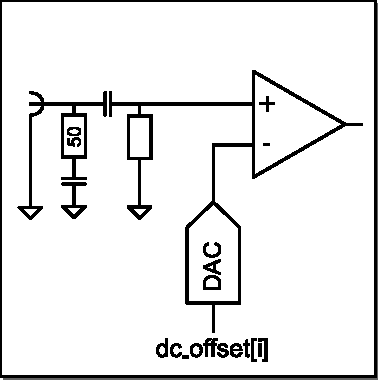
\includegraphics[width=0.3\textwidth]{xhptdc/figures/InputCircuit.pdf}
			}{
				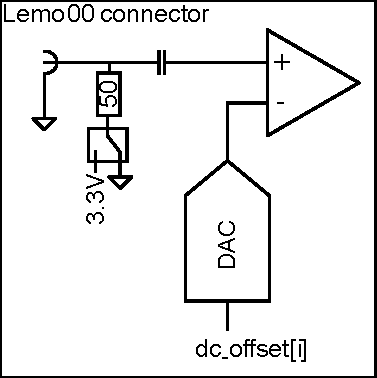
\includegraphics[width=0.3\textwidth]{figures/InputCircuit.pdf}
			}
			\caption{Input circuit for each of the input channels. \label{fig:dcoffset1}}
		\end{center} 
	\end{figure}
%%			\begin{figure}
%%				\begin{center}
%%					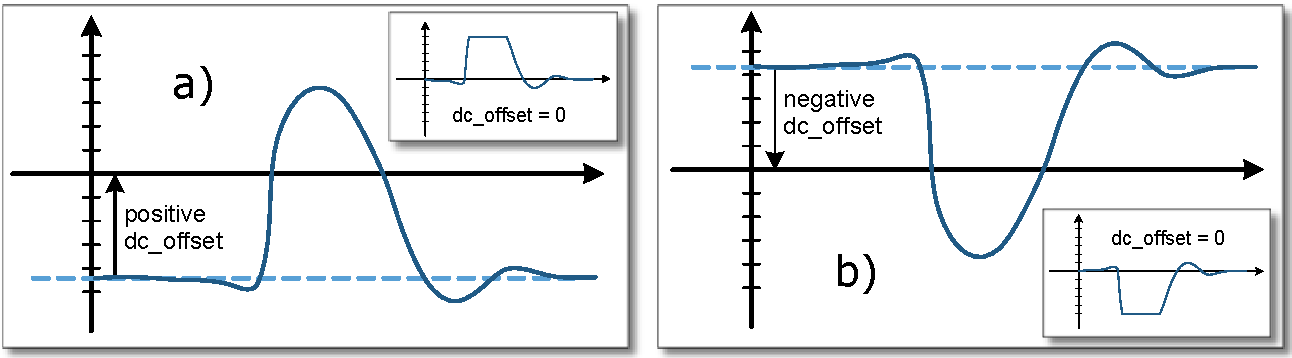
\includegraphics[width=\textwidth]{figures/dc_offset.pdf}
%%%					\caption{\textit{dc\tu offset} is used to shift the signal on each input channel such that the noise margin relative to the switching threshold is maximized.
%%					Insets of figure a) and b) show the base line of the signal with $\mathrm{\textit{dc\tu offset}}~=~0$ close to the switching threshold of the input buffer. Figure a) shows the positive pulse with $\mathrm{\textit{dc\tu offset}}~>~0$ and figure b) shows the negative pulse with $\mathrm{\textit{dc\tu offset}}~<~0$.\label{fig:dcoffset2}}
%%				\end{center}
%%			\end{figure}

	\ttvar{\prefix trigger}{trigger[\PREFIX TRIGGER\tu COUNT]}\\
	Configures the polarity of the external trigger sources.
	These are used as inputs for the TiGer blocks and as inputs to the time measurement unit.\par

	\ttvar{\prefix tiger\tu block}{tiger\tu block[\PREFIX TIGER\tu COUNT]}\\
	Configuration of the timing generators (TiGer).

	\ifxHPTDC{
		\ttvar{\prefix tiger\tu block}{gating\tu block[\PREFIX GATE\tu COUNT]}\\
		Configuration of the gating blocks.	
	}{} % only for xHPTDC8

	\ttvar{\prefix channel}{channel[\PREFIX CHANNEL\tu COUNT]}\\
		Configure the TDC channels.

	\ifxHPTDC{
		\cronvar{crono\tu bool\tu t}{skip\tu alignment}\\
		If set,  the phase of the two TDC chips is not realigned when capturing is restartet.

		\cronvar{crono\tu bool\tu t}{alignment\tu source}\\
		Define a signal source that is used for phase alignment. Should usually be left unchanged.
		\begin{tabular}{ll}
			\ttdef{ALIGN\tu TIGER} & 0\\
			\ttdef{ALIGN\tu PIN} & 1\\
			\ttdef{ALIGN\tu RESERVED} & 2\\
		\end{tabular}\par
		
	}{
		\ttvar{\prefix low-res\tu channel}{low-res\tu channel[\PREFIX LOWRES\tu CHANNEL\tu COUNT]}\\
		\itett{
			Not applicable for \deviceName. 
		}{
			Only applicable to the xTDC4-Sciex. Configures the additional digital low-res inputs.
		}\par
		\autotrigger
	
	}

	

%%%%%%%%% trigger
	\subsection{Structure \prefix trigger}
	\label{structtrigger}
	For each input this structure determines wheter rising or falling edges on the inputs create trigger events for the TiGer \ifxHPTDC{and gating}{} blocks.

	\cronvar{crono\tu bool\tu t}{falling}\\
	\cronvar{crono\tu bool\tu t}{rising}\\
	Select for which edges a trigger event is created inside the FPGA.
	\txh{
		Set the corresponding flag for one of the edges or both edges then using the input with a TiGer.
	}{
		The \deviceName can output measurements with a reduced bin size of $5/6~ns = 833,\overline{3}~ps$ for one or both edges of input signals. 
		See section \ref{difficulthits} for more information on hits with varying resolution.
		Use \textsf{xtdc4\tu channel.rising} on page \pageref{structchannel} to select which edge is measured with full resolution.
		The edge that is selected for full resolution measurement must also be enabled for low resolution measurement.
	}{
		While the TDC can only measure either rising or falling edges, the gating blocks and the TiGer are more flexibel. 
		Set the corresponding flag for one of the edges or both edges when using the input with a TiGer or gating block.
	}\par

%%%%% tiger_block			

	\subsection{Structure \prefix tiger\tu block\label{cp:tigerblock}}
	See section \ref{cp:tiger} for additional information.
	\ifxHPTDC{
		\cronvar{int}{mode}\\*
		Enables the desired mode of operation for the tiger. \\*
		\begin{tabular}{lrl}
			\ttdef{TIGER \tu OFF} & 0 & No operation \\
			\ttdef{TIGER \tu OUTPUT} & 1 & Output is driven with 2V amplitude. \\*
										&   &There must be no input connected \\
			\ttdef{TIGER \tu BIDI} & 2 & Output is driven with 1V amplitude. \\*
									&   & Pulse rate should be low. \\*
			\ttdef{TIGER \tu BIPOLAR} & 3 & Output is driven with 1~V bidirectional pulses.\\*
									&   & $start = stop -1$\\*
		\end{tabular}
		The gating blocks are only used internally and produce no pulses accessible to the user.		
		Gating blocks interpret any value that is not 0 as as enable.\\*
		\begin{tabular}{lrl}
			\ttdef{GATE \tu OFF} & 0 & No gating, alle hits are captured. \\*
			\ttdef{GATE \tu ON} & 1 & No hits are captured while the gate is active.\\*
		\end{tabular}
	
	}{
		\cronvar{crono\tu bool\tu t}{enable}\\
		Activates the timing generator (TiGer).\par
	}

	\cronvar{crono\tu bool\tu t}{negate}\\
	Inverts output polarity. Default is set to false.
	\ifxHPTDC{For gating blocks, a value of false blocks inputs between start and stop, a value of true blocks outputs outside that interval.
	The TiGer creates a high pulse from \textsf{start} to \textsf{stop} unless negated.}{}\par

	\cronvar{crono\tu bool\tu t}{retrigger}\\
	Enables retrigger setting.\\
	If enabled the timer is reset to the value of the \textsf{start} parameter, whenever the input signal is set while waiting to reach the \textsf{stop} time.\par

	\cronvar{crono\tu bool\tu t}{extend}\\
	Not implemented.

	\ifxHPTDC{}{
		\cronvar{crono\tu bool\tu t}{enable\tu lemo\tu output}\\
		Enables the LEMO output. Drive the TiGer Signal to the corresponding Lemo connector as an output. 
		This is DC coupled, so make sure that you do not any devices connected as inputs.
		Pulses created by the TiGer are visible at the \deviceName inputs and can be measured again to get the exact timing.  
	}

	\cronvar{int}{start}\\
	\cronvar{int}{stop}\\
	\itett{
		In multiples of $4~ns$.
	}{
		In multiples of $20~ns/3 = 6,\overline{6}~ns$
	}
	The time during which the TiGer output is set, relative to the trigger input. The parameters \textsf{start} and \textsf{stop} must fulfill the following conditions:
	\[ 0 <= start <= stop <= 2^{16}-1 \]
	If retriggering is enabled, the timer is reset to the value of the start parameter whenever the input signal is set while waiting for the stop time. \par
	

	\cronvar{int}{sources}\\
	A bit mask with a bit set for all trigger sources that can trigger this TiGer block. 
	Default is \textsf{\PREFIX TRIGGER\tu SOURCE\tu \ifxHPTDC{A}{S}}.\par

	\begin{tabular}{lc}
			\ttdef{TRIGGER\tu SOURCE\tu NONE} & 0x00000000\\
		\ifxHPTDC{
			\ttdef{TRIGGER\tu SOURCE\tu A} & 0x00000001\\
			\ttdef{TRIGGER\tu SOURCE\tu B} & 0x00000002\\
			\ttdef{TRIGGER\tu SOURCE\tu C} & 0x00000004\\
			\ttdef{TRIGGER\tu SOURCE\tu D} & 0x00000008\\
			\ttdef{TRIGGER\tu SOURCE\tu E} & 0x00000010\\
			\ttdef{TRIGGER\tu SOURCE\tu F} & 0x00000020\\
			\ttdef{TRIGGER\tu SOURCE\tu G} & 0x00000040\\
			\ttdef{TRIGGER\tu SOURCE\tu H} & 0x00000080\\
			\ttdef{TRIGGER\tu SOURCE\tu TDC1\tu SYNC} & 0x00000100\\
			\ttdef{TRIGGER\tu SOURCE\tu TDC2\tu SYNC} & 0x00000200\\
			\ttdef{TRIGGER\tu SOURCE\tu TDC\tu EXT\tu SYNC} & 0x00000400\\
			\ttdef{TRIGGER\tu SOURCE\tu ADC1\tu CONV} & 0x00000800\\
			\ttdef{TRIGGER\tu SOURCE\tu ADC2\tu CONV} & 0x00001000\\
			\ttdef{TRIGGER\tu SOURCE\tu AUTO} & 0x00004000\\
			\ttdef{TRIGGER\tu SOURCE\tu ONE}  & 0x00008000	
		}{
				\ttdef{TRIGGER\tu SOURCE\tu S} & 0x00000001\\
				\ttdef{TRIGGER\tu SOURCE\tu A} & 0x00000002\\
				\ttdef{TRIGGER\tu SOURCE\tu B} & 0x00000004\\
				\ttdef{TRIGGER\tu SOURCE\tu C} & 0x00000008\\
				\ttdef{TRIGGER\tu SOURCE\tu D} & 0x00000010\\
				\ttdef{TRIGGER\tu SOURCE\tu AUTO} & 0x00004000\\
				\ttdef{TRIGGER\tu SOURCE\tu ONE} & 0x00008000
		}
	\end{tabular} 

%%%%%%%%%%%%%%%%%%%%%%%% channel

	\subsection{Structure \prefix channel}
		\label{structchannel}
		Contains TDC channel settings.\par

		\cronvar{crono\tu bool\tu t}{enable\ifxHPTDC{}{d}}\\
		Enable TDC channel.\par

		\cronvar{crono\tu bool\tu t}{rising}\\
		\txh{
			Not applicable for \deviceName.
		}{
			Select which edge of the signal is used for full resolution measurements. 
			\textsf{xtdc4\tu trigger.rising} and \textsf{xtdc4\tu trigger.falling} described on page \pageref{structtrigger} are used 
			to select which edges are recorded for low resolution measurement. 
			The edge that is selected for full resolution measurement must also be enabled for low resolution measurement.
			See section \ref{difficulthits} for more information on hits with varying resolution.
		}{
			Select which edge of the signal is measured by the TDC. 
			The TiGer and gating blocks use a separate configuration that allows to use both edges simultaneously on each input. See section \ref{structtrigger}
		}\par

		\txh{}{ %only for xTDC4
			\cronvar{crono\tu bool\tu t}{cc\tu enable}\\
			Enable carry chain TDC. This is set to \emph{true} by default and should be left unchanged. \par

			\cronvar{crono\tu bool\tu t}{cc\tu same\tu edge}\\
			Sets whether the carry chain TDC records the same or opposite edge as the TDC chip. 
			If the same edge is selected, that carry chain TDC acts  as a backup if the chip misses hits due to FIFO overflows or short input pulses.
			If opposite edges are selected, both edges of a pulse can be measured with reasonable resolution. See section \ref{difficulthits} for more information.\par

			\cronvar{crono\tu bool\tu t}{ths788\tu disable}\\
			Disable full resolution timestamps. This is set to \emph{false} by default and should be left unchanged.\par
		}{}

		\ifxHPTDC{}{
			\cronvar{int}{start}\\
			\cronvar{int}{stop}\\
			Veto function for grouping of hits into packets in multiples of the binsize. Only hits between start and stop are read out.
			The parameters must adhere to the following relations:
			\[
				0 <= start <= stop < 2^{ \itett{31}{30}}
			\]
		}

%%%%%%%%%%%%%%%%%%%%% grouping, only fpr xHPTDC8

\ifxHPTDC{
	\subsection{Structure \prefix grouping\tu configuration}	
	\label{structgrouping}
	This structure configures the behaviour of the grouping functionality. See section \ref{grouping}.
	Grouping is enabled with the \textsf{tdc\tu mode} paramter defined in the top level of the config structure.

	In this structure intervals are always provided in picoseconds, independently of the bin size of the TDC.

	\cronvar{bool}{enable}
	Enable grouping. Defaults to \textsf{false}.

	\cronvar{int}{trigger\tu channel}\\
	Channel number that is used to trigger the creation of a group.\par

	\cronvar{int}{zero\tu channel}\\
	Optionally a different channel can be used to calculate the relative timestamps in a group. 
	This is disabled per default by setting this paramteer to $-1$.\par
	
	\cronvar{\tu\tu int64}{zero\tu channel\tu offset}\\
	This offset in picoseconds is added to relative timestamps within a group.\par

	\cronvar{\tu\tu int64}{range\tu start}\\
	\cronvar{\tu\tu int64}{range\tu stop}\\
	Values in the interval from \textsf{range\tu start} to \textsf{range\tu stop} are included in the group. 
	Either or both values can be negative to create common-stop behaviour. 
	\[
		-2^{63} \le range\_start \le range\_stop < 2^{63} 
	\]\par

	\cronvar{\tu\tu int64}{trigger\tu deadtime}\\
	After a trigger was detected additional triggers will be suppressed for this interval. Must not be negative.\par

	\cronvar{crono\tu bool\tu t}{require\tu windows\tu hit}\\
	If set a group is only created if there is at least one hit in the window defined by \textsf{window\tu start} and \textsf{window\tu stop}.\par

	\cronvar{\tu\tu int64}{window\tu start}\\
	\cronvar{\tu\tu int64}{window\tu stop}\\
	\[
		-2^{63} \le window\_ start \le window\_ stop < 2^{63} 
	\]\par

	\cronvar{int}{veto\tu mode}\\
	A window defined by \textsf{veto\tu start} and \textsf{veto\tu stop} can be used to suppress hits. 
	The functionality is very similar to the gating blocks but is defined in software. 
	While gating blocks can only work locally on the information available within each board the veto function is applied globally accross all boards.
	This feature can not be used to improve FIFO usage or PCIe bandwidth usage. 
	 \\*
	Either data inside or outside the veto window can be suppressed.\\*
	\begin{tabular}{lc}
		\ttdef{VETO\tu OFF}     & 0 \\
		\ttdef{VETO\tu INSIDE}  & 1 \\
		\ttdef{VETO\tu OUTSIDE} & 2 \\
	\end{tabular}\par

	\cronvar{\tu\tu int64}{veto\tu start}\\
	\cronvar{\tu\tu int64}{veto\tu stop}\\
	\[
		-2^{63} \le veto\_ start \le veto\_ stop < 2^{63} 
	\]\par

	\cronvar{crono\tu bool\tu t}{veto\tu relative\tu zero}\\
	If set, the veto window is defined relative to the zero channel. Otherwise the window is defined relative to the trigger.\par 

	\cronvar{crono\tu bool\tu t}{overlap}\\
	Unsupported, must remain \textsf{false}.

}{}


	%%%%%%%%%%%%%%

	\ifxHPTDC{
       \section{User Data Storage}
	   There is a 64kiByte flash memory on each board that users can utilize to store any type of data. 
	   A typical use case would be calibration data for the \deviceName\ or the detectors that the device is connected to.
	   Also serial numbers of instruments built with the \deviceName\ can be stored here. Write operations allways erase the whole memory block.\par 

	   \ttdef{USER\tu FLASH\tu SIZE 0x10000}\\*     
	   The size of the flash memory in bytes.\\

	   \ttvar{int}{read\tu user\tu flash(\device,  \cronvar{int}{index}, \lb \cronvar{\uchar *}{flash\tu data}, \cronvar{size\tu t size}{size})} \\*
	   \ttvar{int}{write\tu user\tu flash(\device,  \cronvar{int}{index}, \lb \cronvar{\uchar *}{flash\tu data}, \cronvar{size\tu t size}{size})} \\*
	   Read from or write to the user flash of a board identified by \textsf{index}. 
	   \textsf{flash\tu data} must point to a buffer allocated by the user. 
	   \textsf{size} must specify the size of that buffer in bytes. 
	   We recommend to always allocat a buffer of the size of the flash memory given by \textsf{\PREFIX\tu FLASH\tu SIZE} to clarify that allways the full buffer is overwritten.\par
	}{}


	
